\newsection{Appendici}
\subsection{Resoconto delle attività di verifica}
\subsubsection{Riassunto delle attività di verifica}
\paragraph{Revisione dei requisiti}
Durante il periodo successivo alla fine delle stesura di ogni documento, i \emph{verificatori}  hanno provveduto all'attività di verifica. Quest'attività è stato eseguita seguendo le linee guida contenute nelle \emph{Norme di progetto v1.0.0} sezione 3.2.2.
Si sono poi calcolate per i documenti le metriche descritte nel punto 2.2.2.
Infine sono stati verificati i processi seguendo le specifiche contenute nelle \emph{Norme di progetto v1.0.0} sezione 3.2.1 e vi sono state calcolate le metriche contenute nel punto 2.2.1 contenute in questo documento.
\subsubsection{Dettaglio delle verifiche tramite analisi}
\paragraph{Processi}
Il grafico PDCA della fase di Analisi è:
\begin{figure} [H]
	\centering
	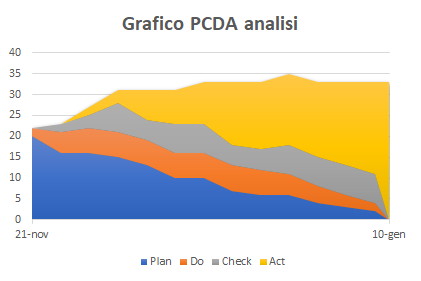
\includegraphics[scale=1]{Img/Grafico_PDCA}
	\caption{Figura n: Grafico PDCA, fase di Analisi}\label{}
\end{figure}
Dal grafico possiamo estrapolare che:
\begin{itemize}
	\item Si notato alcuni mutamenti dei processi pianificati, dovuti ad errori di pianificazione dati dalla poca esperienza del gruppo di lavoro;
	\item Si può notare come il gruppo abbia cercato di rendere omogenea nel tempo l'avanzamento dei processi, alcuni rallentamenti sono dovuti alla sovrapposizione degli impegni
	universitari dei componenti del gruppo con la realizzazione del progetto. Nel complesso si vede come l'omogeneità è stata abbastanza rispettata.
\end{itemize}
\paragraph{Documenti}
Vengono qui riportati i valori dell’indice Gulpease per ogni documento durante la fase
di Analisi. Un documento è considerato valido soltanto se rispetta le metriche descritte
su 4.1.
\begin{longtable}{|c|c|c|}
\hline
\textbf{Documento} & \textbf{Valore indice} & \textbf{Esito} \\
\hline
	\emph{Piano di Progetto v1.0.0} & {???} & {Superato}\\
\hline
	\emph{Norme di Progetto v1.0.0} & {???} & {Superato}\\
\hline
	\emph{Analisi dei Requisiti v1.0.0} & {???} & {Superato}\\
\hline
	\emph{Piano di Qualifica v1.0.0} & {???} & {Superato}\\
\hline
	\emph{Studio di Fattibilità v1.0.0} & {???} & {Superato}\\
\hline
	\emph{Glossario v1.0.0} & {???} & {Superato}\\
\hline
\caption[Tabella n: Esiti verifica documenti, Analisi]{Tabella n: Esiti verifica documenti, Analisi}
\label{tabella:verifica documenti}
\endhead
\end{longtable}
Dalla tabella si può notare come tutti gli indici Gulpease dei documenti rientrino nei vincoli dati e sono di facile lettura anche per chi ha la licenza elementare. Per questo motivo i documenti redatti hanno raggiunto la leggibilità desiderata.
\subsubsection{Dettaglio dell’esito delle revisioni???}
Le revisioni del committente previste durante lo sviluppo del progetto sono quattro.
Al termine di ogni revisione, il committente segnalerà le problematiche riscontrate attraverso una valutazione globale dell'andamento del progetto ed una dettagliata per ciascun documento. 
Questo aiuterà il gruppo a eliminare problemi e criticità nel progetto per poi procedere su una base verificata e il più possibile corretta.
\pagebreak